%
%  Vincent Yannello
%
\documentclass[12pt,fullpage]{article}
\usepackage{fullpage}
\usepackage{psfrag}                                          % LaTeX graphics tool
\usepackage{pslatex}                                         % avoids the default cmr font
\usepackage{graphicx}                                        % graphics package 
\usepackage{epsfig}                                          % figures
\usepackage{hyperref}
\usepackage{color}

\begin{document}

\noindent
{\bf Standard Wald distribution} (from \color{blue}\url{http://www.math.wm.edu/~leemis/chart/UDR/UDR.html}\color{black})

\noindent
The shorthand $X \sim {\rm standard Wald}(\lambda)$ is used to indicate that the
random variable $X$ has the standard Wald distribution with parameter $\lambda$.
A standard Wald random variable $X$ with parameter $\lambda$ has probability density function 
$$
f(x) = \sqrt {{\frac {\lambda}{2 \pi \, {x} ^ {\kern 0.08 em 3}}}}{\kern 0.08 em e ^ {- {\frac {\lambda( x - 1) ^ {2}} {2 x}}}} \qquad \qquad x>0,
$$
for $\lambda > 0$.
The probability density function for two different values of $\lambda$ is illustrated below.
{\begin{figure}[h!]
\begin{center}
\psfrag{lab1}{$\lambda = 0.4$}
\psfrag{lab2}{$\lambda = 3$}
\psfrag{labx}{$x$}
\psfrag{labf}{$f(x)$}
\includegraphics[width=3.2in]{StandardwaldPlot.ps}
\end{center}
\end{figure}}\\
The cumulative distribution function on
the support of $X$ is
$$
F(x) = P(X \le x) = \int _{0} ^ {x} \! \sqrt {{\frac {\lambda}{2\pi \, {t} ^ {\kern 0.08 em 3}}}}{\kern 0.08 em e ^ {- {\frac {\lambda(t - 1) ^ {2}} {2 t}}}} {dt} \qquad \qquad x > 0.
$$
The survivor function, hazard function, inverse distribution, and cumulative hazard functions on the support of $X$ are mathematically intractable.
The moment generating function of $X$ is
$$
M(t) = E\left[ e ^ {tX} \right] = e ^ {\kern 0.08 em \lambda}\left(1 - \sqrt{1 - \frac{2 t}{\lambda}}\right) \qquad \qquad t < \frac{\lambda}{2}.
$$
The characteristic function of $X$ is
$$
\phi(t) = E\left[ e ^ {itX} \right] =  e ^ {\kern 0.08 em \lambda}\left(1 - \sqrt{1 - \frac{2 it}{\lambda}}\right) \qquad \qquad t < \frac{\lambda}{2}.
$$
The population mean, variance, skewness, and kurtosis of $X$ are
$$
E[X] = 1 \qquad \qquad 
V[X] = \frac{1}{\lambda} \qquad \qquad
E\left[ \left( \frac{X - \mu}{\sigma} \right) ^ {\kern -0.08 em 3} \right] = \frac{3}{\sqrt {\lambda}} \qquad \qquad 
E\left[ \left( \frac{X - \mu}{\sigma} \right) ^  {\kern -0.08 em 4} \right] = 3 + \frac{15}{\lambda}.
$$

\vspace{0.1in}

\newpage
\noindent
{\bf APPL verification:}
The APPL statements
\begin{verbatim}
X:=[[x -> sqrt(lambda / (Pi * 2 * x ^ 3)) * exp(-lambda(x - 1) ^ 2 / (2 * x))], 
    [0,infinity], ["Continuous", "PDF"]];
CDF(X);
Mean(X);
Variance(X);
Skewness(X);
Kurtosis(X);
MGF(X);
\end{verbatim}
verify the cumulative distribution function and moment generating function but fail to yield the expected values.
\end{document}
